\chapter{Fundamentação Teórica}
\label{chap:fundteorica}
Nessa parte será apresentados conceitos para melhor entendimento deste trabalho e da modelagem utilizada. 
A próxima seção elucida o que são grafos e, depois, é explicado a variação de grafo utilizado para modelar o problema proposto. Logo em seguida, é esclarecido o ambiente que será abstraído, explicando algumas regras básicas do jogo.
\section{Grafos}
\label{chap:grafos}

De uma maneira resumida e simples, poderia-se dizer que os grafos são a abstração matemática que descreve uma situação utilizando pontos e uma ligação entre alguns destes \cite{Lucchesi1979}.
Um grafo \(G(V, E)\) pode ser definido como um conjunto de vértices \(V\) e seu conjunto de arestas \(E\), sendo que cada elemento \(e \in E\), associa dois vértices do conjunto \(V\). Assim, se os vértices \((u,v) \in E\), então eles \(u\) e \(v\) são conectados pela aresta \(e\) e são considerados como vértices vizinhos ou adjacentes \cite{grafosucinto, Viana2007}.

Os grafos também podem ter suas arestas classificadas como binárias ou ponderadas, sendo os binários suas arestas representadas apenas por 1 ( se existem ) ou 0 ( se não existem ) e as ponderadas quando existe um valor no conjunto \(W\), o qual informa a intensidade da interação de uma aresta entre dois vértices  \cite{Viana2007, cormen6}.
Na Figura \ref{fig:grafo-exemplobinario} temos um grafo binário,  em que se \((u,v) \in E\), então ela está representada no grafo. Ná na Figura \ref{fig:grafo-exemploponderado} além da existência da conexão entre os vértices, está representado o valor da aresta no conjunto \(W\) informando o peso. 

É chamado de grafo orientado quando \((u,v) \in E\) é diferente de \((v,u) \in E\). Neste caso, quando um vértice é ligado ao outro, não necessariamente esse segundo vértice é conectado ao primeiro, como um exemplo mostrado na Figura \ref{fig:grafo-exemploorientado}.
\citet{grafosucinto} afirmam sobre a vizinhança de um grafo que "O conjunto de vértices \(X\) de um grafo \(G\) é o conjunto de todos os vértices que tem algum vizinho em \(X\)", e diz que esse conjunto de vértices pode ser chamado de \(\Gamma_G(X)\). Exemplificando, o conjunto \(\Gamma_G(1)\) da Figura \ref{fig:grafo-exemplobinario} são os vértices \(2\) e \(4\) e a aresta \( (2,4) \) sendo representados na Figura \ref{fig:grafo-vizinhanca}.

\begin{figure}[!h] \centering
	\centering
	\caption{Exemplo de grafos.}
	\subfloat[Grafo binário com quatro vértices e quatro arestas.]{
		\begin{tikzpicture}
		\begin{scope}[xshift=4cm]
		\node[main node] (1) {$1$};
		\node[main node] (2) [right = 2cm  of 1] {$2$};
		\node[main node] (3) [below = 2cm  of 1] {$3$};
		\node[main node] (4) [right = 2cm  of 3] {$4$};
		
		\path[draw,thick]
		(1) edge node {} (2)
		(1) edge node {} (4)
		(4) edge node {} (2)
		(4) edge node {} (3)
		;
		\end{scope}
		\end{tikzpicture}
		\label{fig:grafo-exemplobinario}
	}
	\subfloat[Grafo não-binário com quatro vértices e três arestas.]{
		\begin{tikzpicture}
		
		\begin{scope}[xshift=4cm]
		\node[main node] (1) {$1$};
		\node[main node] (2) [right = 2cm  of 1] {$2$};
		\node[main node] (3) [below = 2cm  of 1] {$3$};
		\node[main node] (4) [right = 2cm  of 3] {$4$};
		
		\draw[-] (1) -- node[above] {2} (2);
		\draw[-] (1) -- node[left] {1} (3);
		\draw[-] (2) -- node[right] {1} (4);
		\end{scope}
		\end{tikzpicture}
		\label{fig:grafo-exemploponderado}
	}

	\subfloat[Grafo não-binário e orientado.]{
		\begin{tikzpicture}
		
		\begin{scope}[xshift=4cm]
		\node[main node] (1) {$1$};
		\node[main node] (2) [right = 2cm  of 1] {$2$};
		\node[main node] (3) [below = 2cm  of 1] {$3$};
		\node[main node] (4) [right = 2cm  of 3] {$4$};
	
		\draw[<->] (1) -- node[above] {2} (2);
		\draw[->] (1) -- node[left] {1} (3);
		\draw[<-] (2) -- node[right] {1} (4);
		\end{scope}
		\end{tikzpicture}
		\label{fig:grafo-exemploorientado}
	}
	\subfloat[Exemplo de vizinhança de um vértice de um grafo.]{
	\begin{tikzpicture}
	\begin{scope}[xshift=4cm]
	\node[targetnode] (1) {$1$};
	\node[main node] (2) [right = 2cm  of 1] {$2$};
	\node[offnode] (3) [below = 2cm  of 1] {$3$};
	\node[main node] (4) [right = 2cm  of 3] {$4$};
	
	\path[draw, style={offline}]
	(1) edge node {} (2)
	(1) edge node {} (4)
	(3) edge node {} (4)
	;
	\path[draw,thick]
	(4) edge node {} (2)
	;
	\end{scope}
	\end{tikzpicture}
	\label{fig:grafo-vizinhanca}	
	}
	\
	\small{\leftline{Fonte: Autor.}}
	\label{fig:grafo-exemplo}
	
\end{figure}



\section{Propriedade topológicas}

O grau de um vértice \(v\),\(g(v)\), é definido sendo a quantidade de arestas que chegam nele. Por exemplo, na Figura \ref{fig:grafo-exemplobinario} vemos que o grau do vértice 1, \(g(1)\), é igual à 2, pois apenas as arestas \((1,2)\) e \((1,4)\) incidem no vértice 1 \cite{grafosucinto}.

O grau máximo de um grafo \(G\) é igual ao do vértice que tem o maior grau presente nesse grafo \(V(G)\), podendo ser expresso por \(\Delta(G) = max\{g(v) : v \in V(G)\}\). O grau mínimo de um grafo, por outro lado, é o grau do vértice com o qual poderíamos escrever por: \(\delta(G) = min\{g(v) : v \in V(G)\}\). um grafo é considerado regular caso \(\delta(G) = \Delta(G)\) e é \(k\)-regular se \(\delta(G) = \Delta(G) = k\) \cite{grafosucinto}.


Os grafos que são modelamos a partir de um sistema real são classificados como redes complexas, as quais veremos na seção seguinte.

\section{Redes Complexas}
\label{chap:redecomplexa}
\citet{Viana2007} afirma que é utilizado o termo redes complexas quando um grafo representa um sistema físico real e, por isso, um grafo do jogo LOL pode ser considerado como uma rede complexa.

Para que seja possível classificar o nosso modelo adequadamente, serão apresentados três modelos que, segundo \citet{albert2002statistical} destacam entre os pesquisadores as redes \textit{small-worlds}, as redes livres de escala e as redes aleatórias.

\subsection{\textit{Redes Small-Worlds}}
 As redes \textit{small-worlds} são um modelo de rede complexas que representa uma alternativa ao modelo aleatório, assumindo como hipótese que redes complexas do mundo real presente no mundo animal, biológico e químico não são completamente aleatórias \cite{watts1998collective, lopes2011redes}. 
 
 Vamos supor que exista um grafo regular com $v$ vértices e $k$ arestas ligando os vizinhos mais próximos e, após de ser formado, cada uma de suas arestas têm uma probabilidade $p$ de se reconectar com outro vértice aleatório. Isto permite que a geração do grafo seja controlada para uma rede regular com $p \approx 0$ ou uma rede aleatória com $p \approx 1$, e, também, a formação de uma rede com topologia intermediária $0 < p < 1$ \cite{lopes2011redes}.
 \begin{figure}[!htb]
 	\caption{Variação do $p$ sem alterar o numero de vértices $v = 20$ e $k = 4$.}
 	\begin{center}
 		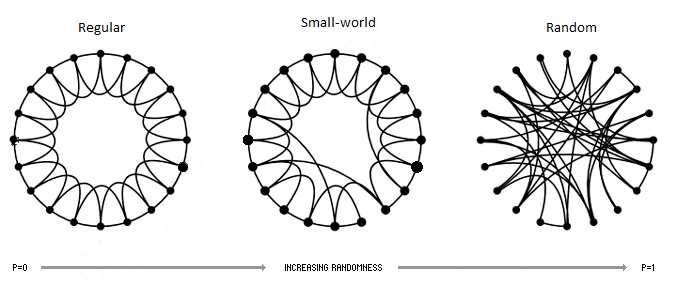
\includegraphics[width=0.9\linewidth]{imagens/watts-sm}
 	\end{center}
 	\small{Fonte: \citet{watts1998collective}.}
 	\label{fig:watts-sm}
 \end{figure} 
 
 As redes \textit{small-worlds} são caracterizadas com duas principais medidas: o tamanho do caminho $L(p)$ e o coeficiente de agrupamento, ou coeficiente de aglomeração, $C(p)$. $L(p)$ é medido como a média do caminho mais curto de todos pares de vértices \cite{lopes2011redes}. O coeficiente de aglomeração será melhor definido na seção \ref{subsec:coeficienteaglomeracao}.
 
 \subsection{Redes Livres de Escala}
 As redes livres de escala, foram propostas por \citet{barabasi1999emergence}, nelas nós possuem probabilidade \(P(k)\) de possuir \(k\) arestas obedecendo a lei da potência \(P(k) \sim k^{-\gamma}\), em que $\gamma$ determina o decaimento exponencial \cite{Antiqueira2005, lopes2011redes}. Segundo \citet{Viana2007}, nas redes livres de escala possuem muitos nós com poucas arestas e poucos nós que se ligam a muitos.
 
A rede livre de escala é baseado em duas regras: crescimento e preferência linear de ligação. A redes é gerada com a inclusão de $n_0 < n$ vértices aleatoriamente conectados, sendo estas inserções antes do crescimento da rede. 
Na etapa de crescimento da rede, um novo vértice $v$ é adicionado na rede a cada instante de tempo $t$, o número de arestas desse vértice segue uma preferencia linear de ligação da fórmula
\[ P(v_i \leftrightarrow v_j) = \frac{k_j}{\sum_u k_U}, \forall v_u \in V .\]

Sendo $P$ a probabilidade de um vértice $v_i$ ser conectado ao novo vértice $v_j$ é linearmente proporcional ao grau $k_j$ do vértice $v_j$  \citet{lopes2011redes}.

 \begin{figure}[!htb]
	\caption{Lei de potência do número de conexões k. De cima pra baixo, as curvas de lei de potência foram obtidas com o parâmetro \(\gamma\) definido como: 0.5 , 1 , 1.5 , 2, 2.5, 3, 4 e 5.}
	\begin{center}
		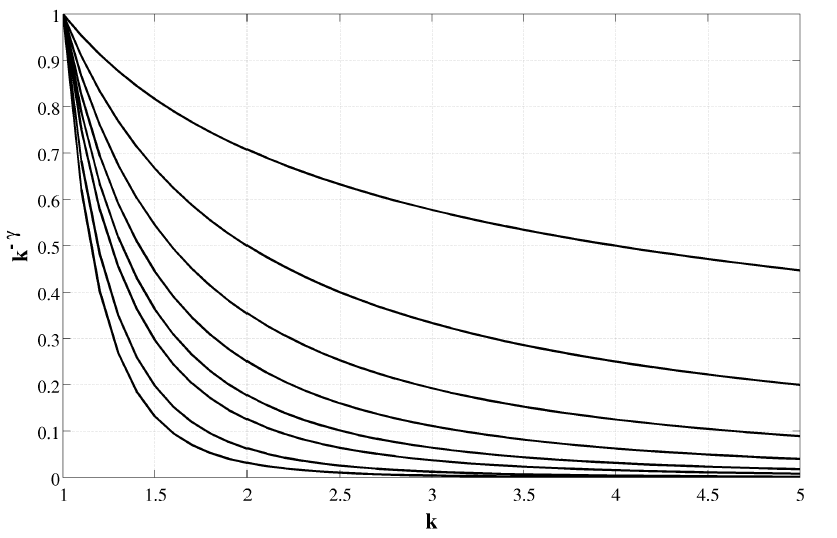
\includegraphics[width=0.95\linewidth]{imagens/scalefree}
	\end{center}
	\small{Fonte: \citet{lopes2011redes}.}
	\label{fig:lei-potencia}
\end{figure} 
 
É possível ver na Figura \ref{fig:lei-potencia} que quanto maior o \(\gamma\), menor a probabilidade de existir vértices com grande número de arestas. O paradigma de ligação dos novos vértices também é conhecido como "o rico fica mais rico" \cite{costa}.
     
\subsection{Redes Aleatórias}
As redes aleatórias, foram inicialmente propostas em 1959 e podem ser consideradas o modelo mais elementar de rede complexas \cite{lopes2011redes, erdds1959random}.
Segundo \citet{Viana2007} e \citet{lopes2011redes}, as redes aleatórias são um sistema formado por $E$ arestas e $N$ vértices que são dispostos inicialmente os vértices e depois aleatoriamente as arestas são distribuídas com probabilidade igual entre os vértices, evitando auto-relacionamentos e conexões múltiplas entre dois vértices.


 
\subsection{Coeficiente de Aglomeração}
\label{subsec:coeficienteaglomeracao}
Segundo \citet{Viana2007}, o coeficiente de aglomeração mede o quão conectado estão os nós da rede ou do grafo. \citet{Antiqueira2005}  definem o coeficiente de aglomeração sendo\[CA_i = \frac{E_i}{k_i(k_i-1)}.\]

\citet{Antiqueira2005}  continua: “Sendo para cada vértice \(i\) existe \(k_i\) arestas, que os ligam a outros \(k_i\) vértices. Se esses \(k_i\) vértices estivessem ligados diretamente à todos os outros vértices do conjunto, haveriam \(k_i(k_i- 1)\) arestas entre eles. E assumindo \(E_i\) o número de arestas que existentes entre os \(k_i\) vértices.	O coeficiente da rede inteira é a média de todos \(CA_i\)”.

\begin{figure}[!h] \centering
	\centering
	\caption{Coeficiente de aglomeração.}
	\subfloat[]{
		\begin{tikzpicture}
		\begin{scope}[xshift=4cm]
		\node[targetnode] (1) {$1$};
		\node[main node] (2) [above right = 2cm  of 1] {$2$};
		\node[main node] (3) [below right = 2cm  of 1] {$3$};
		\node[main node] (4) [right = 2cm  of 2] {$4$};
		\node[main node] (5) [right = 2cm  of 3] {$5$};
		
		\path[draw,thick]
		(1) edge node {} (2)
		(1) edge node {} (3)
		(1) edge node {} (4)
		(1) edge node {} (5)	
		(2) edge node {} (3)
		(2) edge node {} (4)
		(2) edge node {} (5)
		(3) edge node {} (4)
		(3) edge node {} (5)
		(4) edge node {} (5)
		;
		\end{scope}
		\end{tikzpicture}
		\label{fig:grafo-aglomeracao1}
	}
	\subfloat[]{
		\begin{tikzpicture}
		\begin{scope}[xshift=4cm]
		\node[targetnode] (1) {$1$};
		\node[main node] (2) [above right = 2cm  of 1] {$2$};
		\node[main node] (3) [below right = 2cm  of 1] {$3$};
		\node[main node] (4) [right = 2cm  of 2] {$4$};
		\node[main node] (5) [right = 2cm  of 3] {$5$};
		
		\path[draw,thick]
		(1) edge node {} (2)
		(1) edge node {} (3)
		(1) edge node {} (4)
		(1) edge node {} (5)
		(2) edge node {} (4)
		(3) edge node {} (5)
		(4) edge node {} (5)
		;
		\end{scope}
		\end{tikzpicture}
		\label{fig:grafo-aglomeracao2}
	}
	\
	\small{\leftline{Fonte: Autor.}}
	\label{fig:grafo-aglomeracao}
\end{figure}

Na Figura \ref{fig:grafo-aglomeracao1}, tem-se que o peso de todas as arestas é 1 e, por isso, o coeficiente de aglomeração
do vértice em azul é 1.  Já na Figura \ref{fig:grafo-aglomeracao2}, o coeficiente do vértice em azul, segundo a fórmula é $\frac{1}{2}$. 
    


\section{\textit{League of Legends}}
\label{chap:lol}
O jogo \textit{League of Legends} é um jogo classificado como arena de batalha online de multi jogadores (do inglês \textit{Multiplayer Online Battle Arena} ) ou conhecido também como MOBA, que é um estilo de jogo em que duas equipes se enfrentam virtualmente em um campo de batalha e cada jogador controla o seu personagem, mais chamado de herói ou campeão. O objetivo do MOBA é derrotar a equipe adversária destruindo a construção principal da equipe inimiga.

A arena na qual acontece o jogo é uma arena onde, normalmente o mapa inicialmente é  espelhado,  ou  seja, o lado que cada time está não  oferece vantagens  exclusivas.  O mapa é composto  de  três caminhos até a base inimiga.
    
%%preciso conferir se essa foto é acervo, ou é do lol

\begin{figure}[H]
	\caption{Mapa do jogo de \textit{League of Legends}}
	\begin{center}
		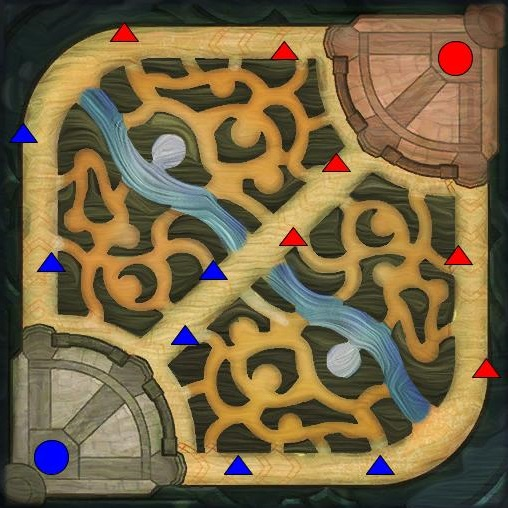
\includegraphics{imagens/mapa_lol.jpg}
	\end{center}
	\small{Fonte: Autor (2018).}
	\label{fig:mapa_lol}
\end{figure}

A Figura \ref{fig:mapa_lol} mostra como é realmente o mapa do jogo, sendo que os círculos mostram a localização da construção principal, e os triângulos as construções de suporte de cada equipe, sendo azul uma equipe e vermelho a outra.
    
No início do jogo cada jogador escolhe  um  herói  diferente, em que  cada  herói tem um conjunto de características únicas, como habilidades especiais que causa uma influência individual no jogo e, indiretamente, na escolha e nos heróis dos outros jogadores, tanto na equipe aliada quanto na equipe inimiga.
    
Depois de escolher os heróis de cada equipe, cada jogador deve procurar adquirir recursos no jogo e meios para conseguir vantagens. Os recursos são limitados por equipe e por tempo, por esse motivo, deve ser bem escolhido quem ficará com a maior parte dos recursos da equipe.
\section{D3.js}
A biblioteca D3.js é uma biblioteca em JavaScript especializada em deixar os dados fáceis de serem lidos e entendidos. Segundo \citet{d3cook}: "Em certo sentido, o D3 é uma biblioteca JavaScript especializada que permite criar incríveis visualizações de dados usando uma abordagem mais simples (baseada em dados), aproveitando os padrões da \textit{Web} existentes", e a organização oficial continua :


\begin{quote}
	O D3.js é uma biblioteca em JavaScript para manipulação de documentos por dados. D3 te ajuda a trazer vida para os dados utilizando HTML, SVG e CSS. A ênfase da biblioteca D3 nos padrões da \textit{web} dá-lhe todos os recursos dos navegadores modernos sem te prender a um \textit{framework} proprietário, combinando poderosos componentes de visualização e uma aproximação orientada por dados da manipulação do DOM.
	\cite[tradução do autor]{d3js}
\end{quote}


Com essa biblioteca é possível dar vida à informações e dados, como, por exemplo, a Figura \ref{fig:d3} que possui duas das diversas maneiras de se exibir informações com o D3.js . Com o D3, foi gerado o grafo do \textit{web service}, programa que será explorado na seção seguinte.

\begin{figure}[!h] \centering
	\centering
	\caption{Coeficiente de aglomeração.}
	\subfloat[]{
		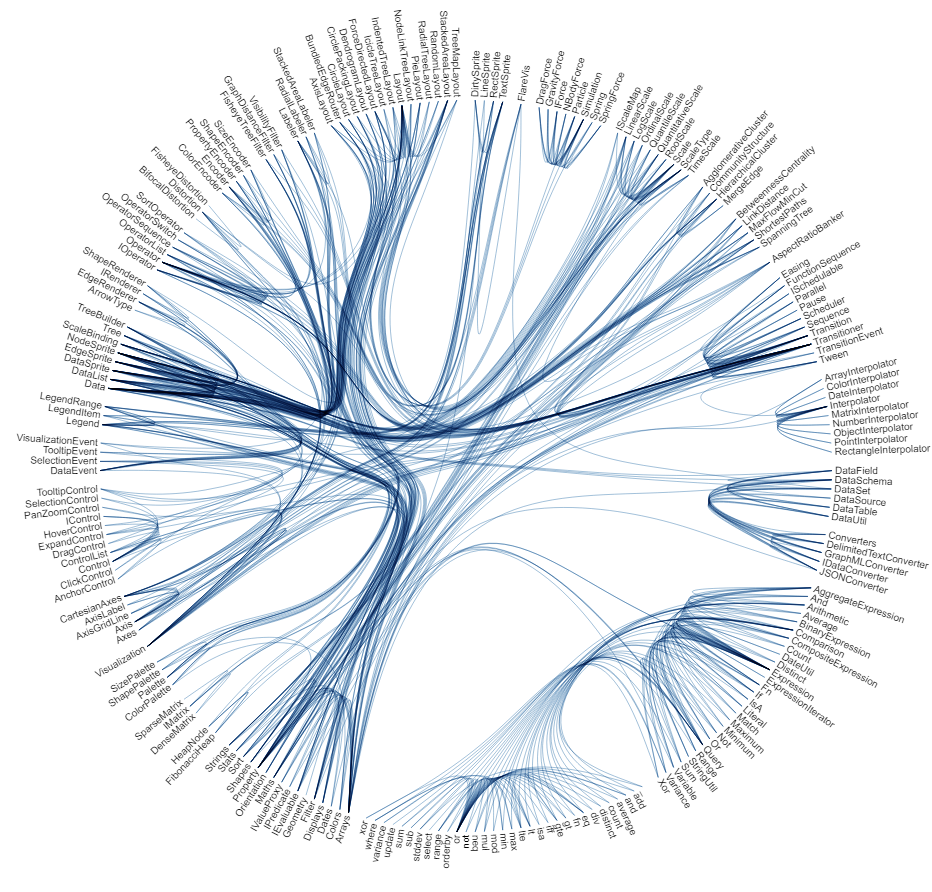
\includegraphics[width=7.5cm]{imagens/d3_1.png}
	}
	\subfloat[]{
		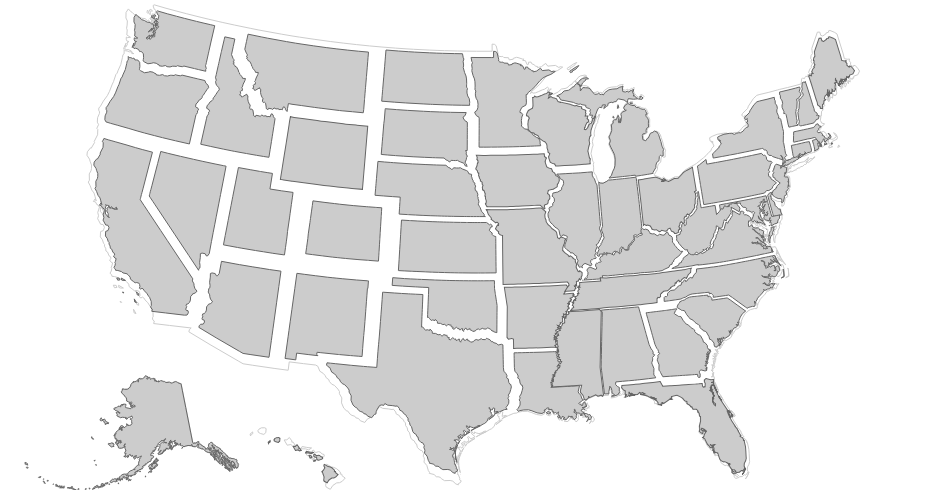
\includegraphics[width=7.5cm]{imagens/d3_2.PNG}%
	}
	\
	\small{Fonte: \cite{d3js}.}
	\label{fig:d3}
\end{figure}


\section{Estado da Arte}


\citet{fbclass} fizeram uma modelação de redes sociais, em que, dados eram adquiridos das redes sociais, e eram modelados em forma de rede complexa. Cada rede complexa depois, passa por processamento de informação, onde são retiradas medidas para estimar a "força" de uma amizade naquela rede social.

\citet{backstrom2006group} também fizeram um trabalho com redes sociais, onde estudam as estruturas das redes sociais MySpace e LiveJournal, e mostraram que até homofilia pode ser usado para melhorar os modelos de predição em um grupo de pessoas.

\citet{dota} com um tema de trabalho também sobre jogos MOBA, fizeram a aquisição de partidas de Dota 2, um jogo da Steam\footnote{https://store.steampowered.com/?l=portuguese}, onde modelam o posicionamento dos jogadores em uma batalha virtual em uma rede complexa, e predizem o vencedor daquela batalha, apenas pelo posicionamento dos jogados.